\chapter{Geschäftswertbeitrag}
\label{Geschaeftswertbeitrag}

\section{Definition}
Der Geschäftswertbeitrag (GWB), im Englischen Economic Value Added (EVA), definiert einen Residualgewinn, welcher eine absolute Nettogröße eines Gewinns nach Abzug der Kapitalkosten für das eingesetze Gesamtkapital ergibt.\footnote{\cite{wikipedia-eva}}

\section{Berechnung}

Der Geschäftswertbeitrag setzt sich aus drei Elementen zusammen: Dem operativen Gewinn nach Steuern (NOPAT - Net Operating Profit After Taxes), das betriebsnotwenige Vermögen (NOA - Net Operating Assets) und die gewichteten durchschnittlichen Kapitalkosten (WACC - Weighted Average Cost of Capital).\\
Der NOPAT ist der Teil, der Operativ entschieden wird. Hierbei geht es darum, dass man das Richtige machen möchte, beziehungsweise etwas besser machen. Die NOA bezieht sich auf eine Entscheidung basierend auf der Investition. Hierbei wird die Verbindlichkeit aus dem laufenden Geschäft nicht berücksichtig, ebenfalls das Ergebnis der Finanzierungstätigkeit. Zuletzt gibt es noch die Finanzierungsentscheidung, welches durch das WACC repräsentiert wird. Zudem kann das WAAC eine gesicherte Aussage über das Unternehmensrisiko geben.\footnote{\cite{bwllexicon-eva}} \footnote{\cite{wikipedia-eva}}\\
In folgender Abbildung \ref{fig:zsmgeschaeftswertbeitrag}\footnote{Quelle: \url{https://www.bwl-lexikon.de/app/uploads/economic-value-added.png}} sind die drei Bestandteile des Geschäftswertbeitrag im Zusammenhang grafisch dargestellt:

\begin{figure}[!h]
    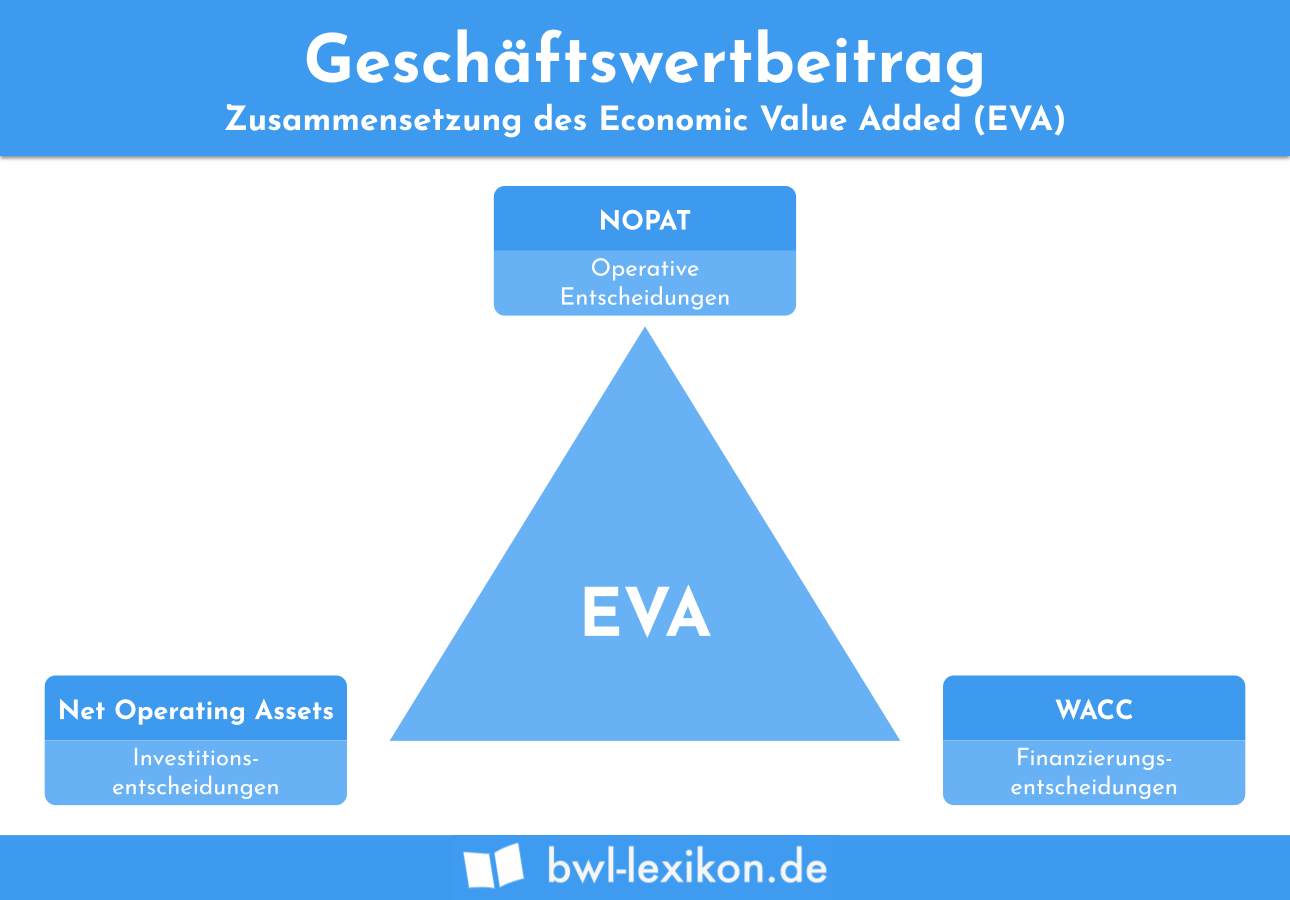
\includegraphics[width=\linewidth]{./media/economic-value-added.png}
    \caption{Zusammensetzung Geschäftswertbeitrag}
    \label{fig:zsmgeschaeftswertbeitrag}
\end{figure}

\subsection{Subtraktiver Ansatz}

Bei dem substraktiven Ansatz werden von dem operativen Jahresergebnis die durchschnittlichen Kapitalkosten mal dem betriebsnotwenigem Vermögen abgezogen. Folgende Formel \eqref{eq:subtraktiver-geschaeftswertbeitrag}\footnote{\cite{wikipedia-eva}} repräsentiert diese Rechnung:

\begin{equation}
    GWB = NOPAT - WACC \cdot NOA
    \label{eq:subtraktiver-geschaeftswertbeitrag}
\end{equation}

\subsection{Multiplikativer Ansatz}

Bei dem multiplikativen Ansatz werden von der Investitionsrendite (ROCE - return on capital employed) die durchschnittlichen Kapitalkosten abgezogen und auf dieses Ergebnis wird dann das betriebsnotwenige Vermögen multipliziert. Dies wird in folgender Formel \eqref{eq:mupliplikativ-gwb-geschaeftswertbeitrag}\footnote{\cite{wikipedia-eva}} dargestellt. In der Formel \eqref{eq:mupliplikativ-roce-geschaeftswertbeitrag}\footnote{\cite{wikipedia-eva}} wird die berechnung der ROCE für die Vollständigkeit dargestellt.

\begin{equation}
    GWB = (ROCE - WACC) \cdot NOA
    \label{eq:mupliplikativ-gwb-geschaeftswertbeitrag}
\end{equation}

\begin{equation}
    ROCE = \frac{NOPAT}{NOA}
    \label{eq:mupliplikativ-roce-geschaeftswertbeitrag}
\end{equation}

\section{Beispielrechnung}

\subsection{Subtraktiver Ansatz}

\subsection{Multiplikatover Ansatz}

\section{Bewertung}
